\documentclass[a4paper, 12pt, final, garamond]{book}
\usepackage{cours-preambule}

\raggedbottom

\makeatletter
\renewcommand{\@chapapp}{Travaux pratiques -- TP}
\makeatother

\let\SavedIndent\indent
\protected\def\indent{%
  \begingroup
    \parindent=\the\parindent
    \SavedIndent
  \endgroup
}
\setlength{\parindent}{0pt}

\begin{document}
\setcounter{chapter}{1}

\chapter{Formation et observation d'images \`a distance finie~: mesures de
distances}

\section{Objectifs}

\begin{itemize}
    \item Réaliser des alignements sur un banc d'optique.
    \item Utiliser un viseur à frontale fixe pour :
        \begin{enumerate}
            \item Réaliser des pointés transversaux permettant de mesurer des
                dimensions d'objet (orthogonaux à l'axe optique).
            \item Réaliser des pointés longitudinaux permettant de mesurer des
                distances entre objets suivant l'axe optique.
            \item Vérifier la formule de Descartes des lentilles.
            \item Vérifier la méthode de Bessel.
            \item Utiliser et apprendre à lire une vis micrométrique.
        \end{enumerate}
\end{itemize}

\section{S'approprier}

\subsection{Principe de fonctionnement d'un viseur à frontale fixe}

\begin{wrapfigure}[5]{r}{0.4\textwidth} 
    \vspace*{-40pt}
    \begin{center}
        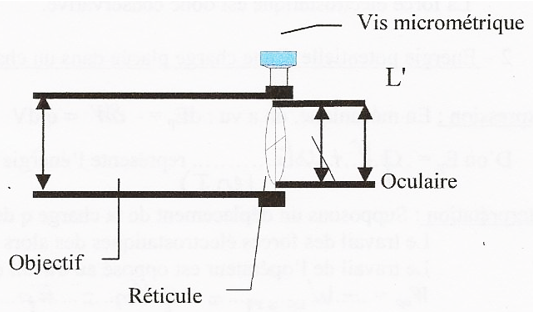
\includegraphics[width=0.4\textwidth]{dispositif}
    \end{center}
\end{wrapfigure} 

Un viseur à frontale fixe est constitué : 

\begin{itemize}
    \item d'un objectif
    \item d'un réticule
    \item d'un oculaire
    \item d'une vis micrométrique permettant de translater le réticule selon un
        axe orthogonal à l'axe optique.
\end{itemize}

L'objectif forme l'image $A'B'$ de $AB$ dans le plan focal objet de l'oculaire,
tel que l'image finale est à l'infini, permettant pour l'œil une observation
sans accommodation. Le réticule est dans ce même plan et est donc visible
simultanément à l'objet $AB$. Globalement, le système peut être représenté par
trois lentilles minces convergentes (dont le cristallin de l'œil) selon 

\centers{$AB  \xrightarrow[\text{objectif}]{} A'B'
    \xrightarrow[\text{oculaire}]{}
    \underbrace{A''B''}_{\infty}\xrightarrow[\text{cristallin}]{} \text{image sur
la rétine}$}

\centers{
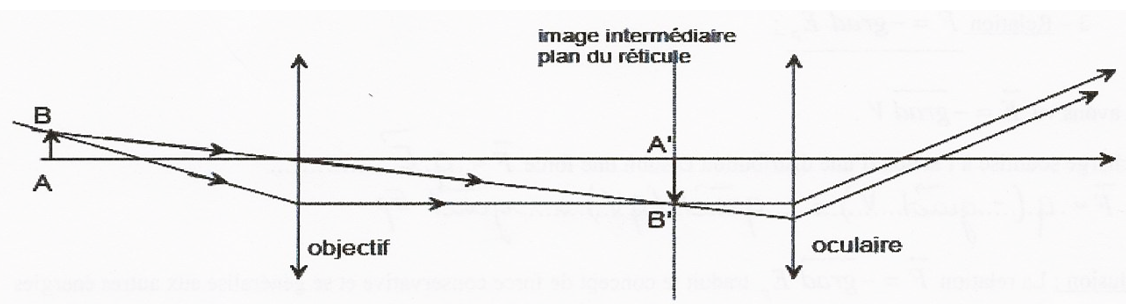
\includegraphics[width=1\linewidth]{schemaDePrincipe}
}

\begin{instruc}{À comprendre}
    Un réticule est placé dans le plan focal objet de l'oculaire. Ainsi, il
    convient de translater le viseur sur le banc optique par rapport à l'objet
    pour voir simultanément l'objet et le réticule net. Nous noterons $D$ la
    distance séparant le centre optique de l'objectif de l'objet visé $AB$.
    Cette distance est fixe, ce qui explique la dénomination de viseur à
    frontale fixe.
\end{instruc}

\subsection{Principe de lecture d'une vis micrométrique}

La vis micrométrique permet de déplacer un double fil vertical dans le plan du
réticule. La vis a un pas (translation réalisée pour un tour complet) de
$\SI{0,5}{mm}$ qui correspond à $50$ graduations du tambour. On peut ainsi en
déplaçant le fil vertical du réticule, mesurer la dimension de l'image $A'B'$
réalisée de l'objet $AB$ au $\SI{1/100}{mm}$.

\begin{figure}[h]
    \centering
    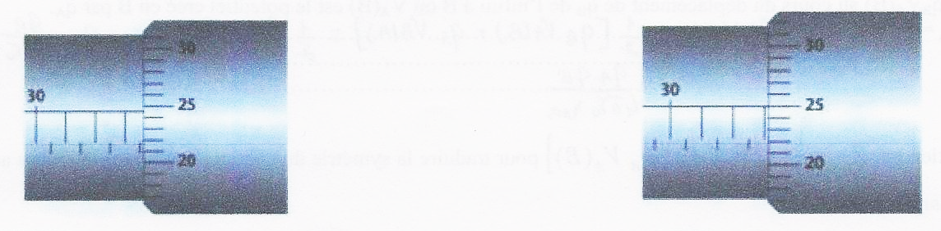
\includegraphics[width=0.7\linewidth]{vis_micro}
    \captionsetup{justification=centering}
    \caption{Principe de lecture sur une vis micrométrique. Un tour complet
    correspond à $\SI{0,5}{mm}$.}
    \label{fig:vis_micro}
\end{figure}

La lecture de gauche donne : $33+\num{0,5}+\num{0,245} = \SI{33,745}{mm}$.\\
La lecture de droite donne : $33+\num{0,250} = \SI{33,250}{mm}$.

\begin{enumerate}
    \item Quelle est l'incertitude-type sur une telle mesure ? (s'aider de la
        fiche pratique sur la théorie de la mesure).
\end{enumerate}

\subsection{Principe de réalisation d'un pointé longitudinal avec un viseur}

On cherche à déterminer la distance algébrique longitudinale $d = \obar{A_1A_2}$
séparant deux objets sur le banc optique. L'objet $A_1B_1$ est constitué par
exemple par la lettre $F$ et l'objet $A_2B_2$ par un quadrillage dessiné sur
feuille transparente. On séparera les deux objets d'une quinzaine de
centimètres. On éclaire l'ensemble avec la lanterne (en $\SI{6}{V}$ alternatif)
devant laquelle on interpose un écran dépoli pour limiter le flux lumineux. 


La première étape consiste à régler le viseur. Pour cela, on translate
l'oculaire en agissant sur l'œilleton de l'oculaire afin de mettre au point le
réticule (c'est-à-dire voir les fils croisés nets). Ce réglage dépend de chacun,
aussi il faut donc en théorie le réaliser à chaque fois que l'observateur
change. En pratique, si votre œil est sans défaut, ou si ces défauts ont été
corrigés, il n'est pas nécessaire de modifier les réglages pour chacun des
membre du binôme. 

\bigskip

La mesure se déroule en deux étapes : 

\begin{enumerate}[label=\alph*)]
    \item Viser l'objet $A_1B_1$ (viser signifie voir l'image nette de l'objet à
        travers le viseur). L'abscisse du viseur est alors :\\
        \centers{$x_{v}(A_1B_1) = x_{A_1}+D$}

    \item Viser l'objet $A_2B_2$. On a alors\\
        \centers{$x_{v}(A_2B_2) = x_{A_2}+D$}
\end{enumerate}

On en déduit alors la distance $d = \obar{A_1A_2}$ comme étant : 

\centers{$x_{v}(A_2B_2) - x_{v}(A_1B_1) = (x_{A_2}+D) - (x_{A_1}+D) = x_{A_2} -
x_{A_1} = d$}

\begin{NCrema}[width=\linewidth]{Remarque} Évidemment, dans la situation
    présente, la méthode semble un peu artificielle, puisqu'il est possible de
    lire directement sur le banc optique la position des objets. Néanmoins, dans
    une situation plus réaliste, une telle méthode peut s'avérer très utile
    puisqu'il devient alors possible de déterminer de loin la distance séparant
    deux objets. 
\end{NCrema}

\subsection{Focométrie~: rappel TP précédent (Bessel et Silbermann)}

\begin{NCdemo}[width=\linewidth]{Rappel}
    La focométrie consiste à déterminer expérimentalement la distance focale
    d'une lentille $(\mathcal{L})$ inconnue. 
\end{NCdemo}

\begin{wrapfigure}[6]{r}{0.3\textwidth} 
    \vspace*{-37pt}
    \begin{center}
        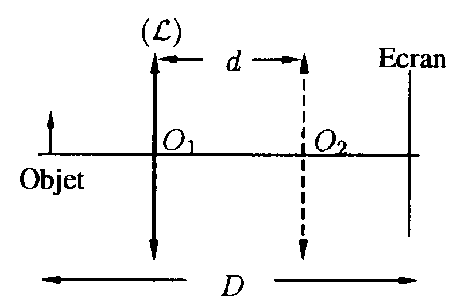
\includegraphics[width=0.3\textwidth]{methodeDeBessel}
    \end{center}
\end{wrapfigure} 

À l'aide d'une lentille mince convergente $(\mathcal{L})$ de distance focale
image $f'$ inconnue, on veut former l'image d'un objet réel sur un écran situé à
une distance $D$ de l'objet. En déplaçant la lentille, on trouve deux positions
$O_1$ et $O_2$ qui donnent une image nette sur l'écran (cf.\ figure ci-contre) à
condition que $D \geq 4f'$. On a vu qu'alors la focale image $f'$ pouvait
s'écrire~: 

\centers{$f' = \dfrac{D^2-d^2}{4D}$} 

La méthode de Silbermann est le cas particulier où $x_1 = x_2$.
\begin{enumerate}[start=2]
    \item Rappeler le principe de cette méthode.
\end{enumerate}

\section{Réaliser et valider un pointé longitudinal avec un viseur}

Suivre le protocole permettant de réaliser un pointé longitudinal et
\textbf{valider} la méthode. Comparer pour ce faire la distance obtenue par
pointé avec le viseur à la distance réelle entre les deux objets (lue
directement sur le banc optique). En déduire l'erreur relative. 

\section{Réaliser et valider un pointé transversal avec un viseur}
\subsection{Mesure du grandissement transversal du viseur}

\begin{wrapfigure}{r}{0.62\textwidth} 
    \begin{center}
        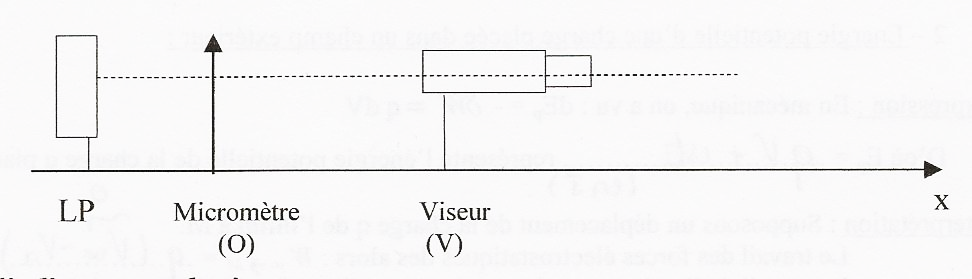
\includegraphics[width=0.6\textwidth]{PointeTransversal}
    \end{center}
\end{wrapfigure} 

Le but de cette première manipulation est de déterminer le grandissement
transversal de l'objectif du viseur : $\gamma = \obar{A'B'}/\obar{AB}$. Pour
cela, on détermine grâce à la vis micrométrique du viseur, la dimension de
l'image $A'B'$ d'un objet $AB$ de dimension connue. L'objet $AB$ de dimension
connue est un micromètre, c'est-à-dire un axe gradué où $100$ traits
représentent $\SI{1}{cm}$. Le micromètre doit être horizontal. Réaliser le
montage ci-contre. Avant toute mesure, il faut régler l'alignement des
instruments d'optique.

\medskip

Approcher le viseur près du micromètre, vérifier les alignements des
instruments, puis s'en écarter tout doucement jusqu'à voir net le micromètre
dans le viseur en superposition avec le réticule.

\begin{enumerate}
    \item Grâce à la vis micrométrique, déplacer le fil vertical mobile du
        réticule sur une graduation centrale du micromètre et noter l'indication
        de la vis.
    \item Faire précisément 2 tours avec la vis micrométrique : Cela représente
        un déplacement de $\SI{1}{mm}$ côté image.
    \item Relever, dans le viseur, la nouvelle graduation du micromètre pointée
        par le fil vertical mobile.
    \item Déduire de ces relevés la valeur absolue du grandissement
        $\abs{\gamma}$ de l'objectif du viseur.
    \item Sachant que l'objectif du viseur est constitué d'une lentille
        convergente, en déduire le grandissement algébrique $\gamma$ de
        l'objectif du viseur.
\end{enumerate}

\subsection{Détermination de la largeur du fil de cuivre}

Prendre comme objet un fil de cuivre, le viseur, positionner correctement le fil
vertical du réticule et, connaissant le grandissement de l'objectif du viseur,
en déduire l'épaisseur de celui-ci.

%\subsection{\'Evaluation de la distance frontale du viseur}
%
%%\'Evaluer la distance focale de la lentille constituant le viseur, en mesurant la distance frontale $D$ (entre ce qu'on vise et le viseur) avec un réglet. Exprimer f' en fonction de ? et D. Faire l'application numérique.

\section{Valider la formule de conjugaison de Descartes}

\subsection{Montage}

\begin{wrapfigure}[4]{r}{0.62\textwidth} 
    \vspace*{-40pt}
    \begin{center}
        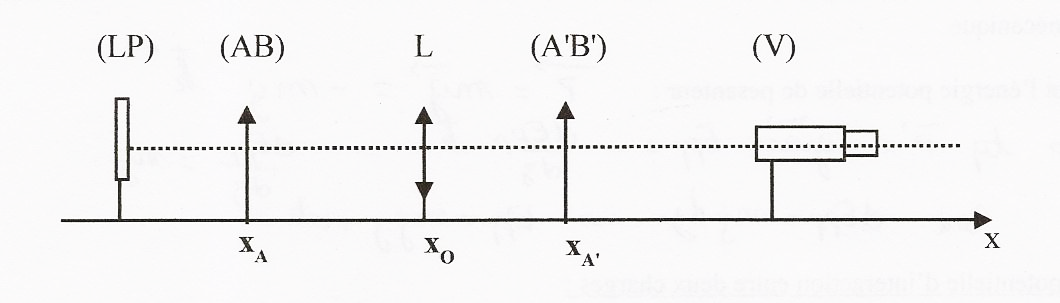
\includegraphics[width=0.6\textwidth]{pointeLongitudinal}
    \end{center}
\end{wrapfigure} 

Prendre comme objet $AB$ la plaque constituée des lettres $F$ sur papier
translucide et réaliser le montage ci-contre avec une lentille convergente de la
focale de votre choix.

\subsection{Mesures}

 Chercher la position approximative de l'image $A'B'$ de $AB$ ainsi obtenue
 grâce à un écran. Viser ensuite cette image $A'B'$ avec le viseur. Noter
 l'abscisse $x_1 = x_{A'} + D$ du viseur sur le banc. Mettre un petit morceau de
 papier sur la lentille $\mathcal{L}$, viser celle-ci avec le viseur en
 réalisant la mise au point sur les déchirures du papier. Noter l'abscisse $x_2
 = x_0 + D$ du viseur sur le banc. Viser enfin l'objet $AB$ avec le viseur
 (après avoir ôté la lentille). Noter l'abscisse $x_3 = x_{A} + D$ du viseur sur
 le banc. Déduire des mesures $\obar{OA}$ et $\obar{OA'}$ en fonction de $x_1$,
 $x_2$ et $x_3$. Faire les applications numériques et à l'aide de la formule de
 conjugaison avec origine au centre des lentilles minces, calculer  $f_{\rm
 exp}'$. Calculer l'écart relatif entre $f_{\rm exp}'$ et $f_{\rm th}'$
 (distance focale indiquée sur la lentille).

\subsection{Observation d'une image virtuelle}

Proposer et réaliser un protocole permettant d'observer à l'aide du viseur une
image virtuelle avec la lentille $V = \SI{-10}{\delta}$ .
Quelles sont les contraintes à respecter ? 
Faire constater votre montage (réussi) par le professeur. 

\section{Focométrie par la méthode de Bessel avec un viseur}

Le viseur joue alors le rôle de l'écran dans la méthode de Bessel telle que vue dans la partie théorique II.D.1. 

\begin{enumerate}
    \item Fixer la position de l'objet $AB$.
    \item Pointer l'objet $AB$ avec le viseur et noter $x_0$ l'abscisse du
        viseur.
    \item Interposer la lentille $\SI{8}{\delta}$ entre l'objet et le viseur.
    \item Déplacer le viseur d'une distance $D > 4f '$ simple et facile à
        repérer. L'abscisse du viseur est alors $x_0 + D$.
    \item Déterminer les positions de la lentille $O_1$ et $O_2$ qui réalisent
        la conjugaison objet image en déplaçant la lentille entre l'objet et le
        viseur, afin d'obtenir une image nette à travers le viseur. Relever les
        deux positions correspondantes de la lentille notées $x_1$ et $x_2$. 
    \item Calculer $d = x_2-x_1$, puis en déduire $f'$.
    \item Appliquer la méthode de Silbermann pour obtenir $f'$ par une autre
        méthode. 
    \item Comparer les valeurs de $f'$ obtenues expérimentalement par chacune
        des méthodes avec la valeur donnée sur la monture de la lentille. 
\end{enumerate}

% \begin{programme}{}
% 
% \begin{itemize}
% \item Mesure de longueurs : sur un banc d'optique. 
% \item Mettre  en œuvre  une  mesure  de  longueur  par 
% déplacement du viseur entre deux positions. 
% \item Utiliser  un  viseur  à  frontale  fixe,  une  lunette  auto-collimatrice. 
% \item Utiliser  des  vis  micrométriques  et  un  réticule  pour 
% tirer  parti  de  la  précision  affichée  de  l'appareil 
% utilisé. 
% \end{itemize}
% \end{programme}
\end{document}
